\documentclass[12pt,titlepage]{article}
\usepackage[margin=1.25in]{geometry}
\usepackage{graphicx,amsmath,minted}
\usepackage{pgf-umlcd}

%% Variables definition
\newcommand{\vSubject}{Object Oriented Programming}
\newcommand{\vSubtitle}{Quiz 1}
\newcommand{\vName}{Dicha Zelianivan Arkana}
\newcommand{\vNIM}{2241720002}
\newcommand{\vClass}{2i}
\newcommand{\vDepartment}{Information Technology}
\newcommand{\vStudyProgram}{D4 Informatics Engineering}

%% [START] Tikz related stuff
\usepackage{tikz}
\usetikzlibrary{svg.path,calc,shapes.geometric,shapes.misc}
\tikzstyle{terminator} = [rectangle, draw, text centered, rounded corners = 1em, minimum height=2em]
\tikzstyle{preparation} = [chamfered rectangle, chamfered rectangle sep=0.75em, draw, text centered, minimum height = 2em]
\tikzstyle{process} = [rectangle, draw, text centered, minimum height=2em]
\tikzstyle{decision} = [diamond, aspect=2, draw, text centered, minimum height=2em]
\tikzstyle{data}=[trapezium, draw, text centered, trapezium left angle=60, trapezium right angle=120, minimum height=2em]
\tikzstyle{connector} = [line width=0.25mm,->]
%% [END] Tikz related stuff

%% [START] Fancy header related stuff
\usepackage{fancyhdr}
\pagestyle{fancy}
\setlength{\headheight}{15pt} % compensate fancyhdr style
\fancyhead{}
\fancyfoot{}
\fancyfoot[L]{\thepage}
\fancyfoot[R]{\textit{\vSubject - \vSubtitle}}
\renewcommand{\footrulewidth}{0.4pt}% default is 0pt, overline for footer
%% [END] Fancy header related stuff

%% [START] Custom tabular command related stuff
\usepackage{tabularx}
\newcommand{\details}[2]{
    #1 & #2  \\
}
%% [END] Custom tabular command related stuff

%% [START] Figure related stuff
\newcommand{\image}[3][1]{
    \begin{figure}[h]
        \centering
        \includegraphics[#1]{#2}
        \caption{#3}
        \label{#3}
    \end{figure}
}
%% [END] Figure related stuff

\begin{document}
\begin{titlepage}
    \centering
    \vfill
    {\bfseries\LARGE
        \vSubject\\
        \vskip0.25cm
        \vSubtitle
    }
    \vfill
    
\includegraphics[width=6cm]{images/polinema-logo.png}
    \vfill
    {
        \textbf{Name}\\
        \vName\\
        \vskip0.5cm
        \textbf{NIM}\\
        \vNIM\\
        \vskip0.5cm
        \textbf{Class}\\
        \vClass\\
        \vskip0.5cm
        \textbf{Department}\\
        \vDepartment\\
        \vskip0.5cm
        \textbf{Study Program}\\
        \vStudyProgram
    }
\end{titlepage}

\section*{Quiz 1}
\subsection*{Class and Object}
\begin{itemize}
    \item {
        What does the word \textbf{class} mean in object-oriented programming?

        A \textbf{class} is a blueprint for creating objects (a particular data structure) which
        can contain states and behaviours. In other words, a class is a template or blueprint
        about the capability of what an object can do.
    }
    \item {
        How do you define an object of a class in Java programming language?

        To define an object of a class in Java programming language, we can use the following
        syntax:

        \begin{minted}[autogobble]{java}
            ClassName objectName = new ClassName();
        \end{minted}

        This process is also known as \textit{instantiation}.
    }
    \item {
        Suppose you have a class \texttt{Item} in an inventory system. How would you make
        a \texttt{laptop} object from that class?

        To make a \texttt{laptop} object from the \texttt{Item} class, we can use the following
        syntax:

        \begin{minted}[autogobble]{java}
            Item laptop = new Item();
        \end{minted}
    }
\end{itemize}

\subsection*{Encapsulation}
\begin{itemize}
    \item {
        Explain the concept of encapsulation in object-oriented programming and its importance
        in the development in an inventory system.

        Encapsulation is a mechanism to hide data from the outer world. It is a way to achieve
        data hiding in Java because other class will not be able to access the data through the
        private data members. The outer world can only access / modify them through the provided
        getter and setter methods.

        It is important to use encapsulation in the development of an inventory system because
        it can protect the data from unwanted changes. In other words, it prevents an object
        from having an invalid or inconsistent state.
    }
    \item {
        In the context of inventory system, mention an example of an attribute that should be encapsulated
        and explain why.

        An example of an attribute that should be encapsulated is the \texttt{stock} attribute.
        We need to have a setter method for this attribute to prevent the stock from having a
        negative value.
    }
\end{itemize}

\subsection*{Class Relationship}
\begin{itemize}
    \item {
        What does it mean by \textbf{class relationship} in object-oriented programming?

        Class relationship is a way of describing how objects are related to each other.
        A class can contain another class as a field. This is known as \textbf{composition}.
        Other type of class relationship is \textbf{inheritance}.
    }
    \item {
        In an inventory system, how would you describe the relation between the class \texttt{Item} and
        \texttt{Category}?

        The relation between the class \texttt{Item} and \texttt{Category} is \textbf{composition}.
        An item can have a category, but a category cannot have an item. It can be illustrated as such:

        \begin{figure}[h]
            \centering
            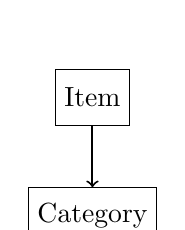
\begin{tikzpicture}
                \node (item) [process] {Item};
                \node (category) [process, below of=item, yshift=-5mm] {Category};
                \draw [connector] (item) -- (category);
            \end{tikzpicture}
            \caption{Class relationship between \texttt{Item} and \texttt{Category}}
            \label{fig:uml-item-category}
        \end{figure}
    }
\end{itemize}

\subsection*{PBL}
\begin{itemize}
    \item {
        Based on the case study of the inventory system, try to create a single class along with its
        attributes and methods that describe an entity in the case study. For example, the class \texttt{Item}.

        \begin{minted}[autogobble,fontsize=\footnotesize]{java}
            public class Item {
                private String name;
                private String description;
                private int stock;

                public Item(String name, String description, int stock, int price) {
                    this.name = name;
                    this.description = description;
                    this.stock = stock;
                }

                public String getName() {
                    return name;
                }

                public void setName(String name) throws IllegalArgumentException {
                    if (name == null) {
                        throw new IllegalArgumentException("Name cannot be null");
                    }
                    if (name.length() < 3) {
                        throw new IllegalArgumentException("Name must be at least 3 characters long");
                    }
                    this.name = name;
                }

                public String getDescription() {
                    return description;
                }

                public void setDescription(String description) throws IllegalArgumentException {
                    if (description == null) {
                        throw new IllegalArgumentException("Description cannot be null");
                    }
                    if (description.length() < 10) {
                        throw new IllegalArgumentException(
                            "Description must be at least 10 characters long"
                        );
                    }
                    this.description = description;
                }

                public int getStock() {
                    return stock;
                }

                public void setStock(int stock) {
                    if (stock < 0) throw new IllegalArgumentException("Stock cannot be negative");
                    this.stock = stock;
                }
            }
        \end{minted}

        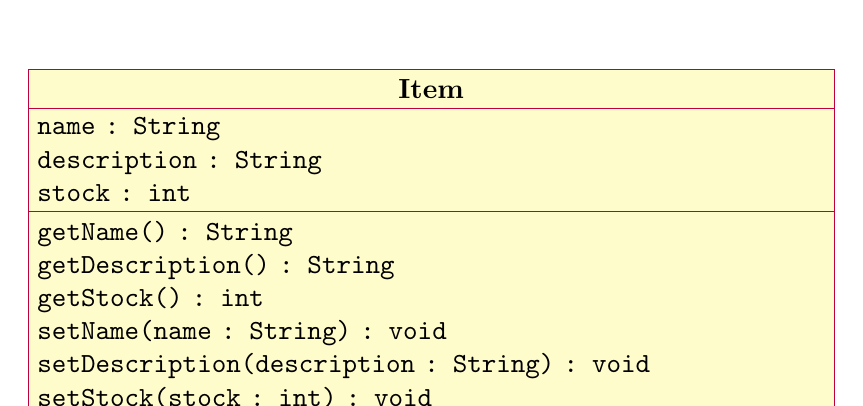
\begin{tikzpicture}
            \begin{class}[text width=10cm]{Item}{0,0}
                \attribute{\texttt{name : String}}
                \attribute{\texttt{description : String}}
                \attribute{\texttt{stock : int}}
                \operation{\texttt{getName() : String}}
                \operation{\texttt{getDescription() : String}}
                \operation{\texttt{getStock() : int}}
                \operation{\texttt{setName(name : String) : void}}
                \operation{\texttt{setDescription(description : String) : void}}
                \operation{\texttt{setStock(stock : int) : void}}
            \end{class}
        \end{tikzpicture}
    }
    \pagebreak
    \item {
        How would you use \textit{encapsulation} to protect the class that you've created?

        We can use \textit{encapsulation} to protect the class that we've created by making the
        attributes private and provide getter and setter methods for them.
        This is used to guard against invalid or inconsistent state of an object. For example,
        the field \texttt{name} and \texttt{description} cannot be null and must be at least
        3 and 10 characters long respectively. The field \texttt{stock} cannot be negative.
    }
    \item {
        Give an example of a \textit{class relationship} in the inventory system.

        An example of a \textit{class relationship} in the inventory system is the relationship
        between the \texttt{Item} and \texttt{Category} class. An item can have a category, but
        a category cannot have an item. It can be illustrated as such:

        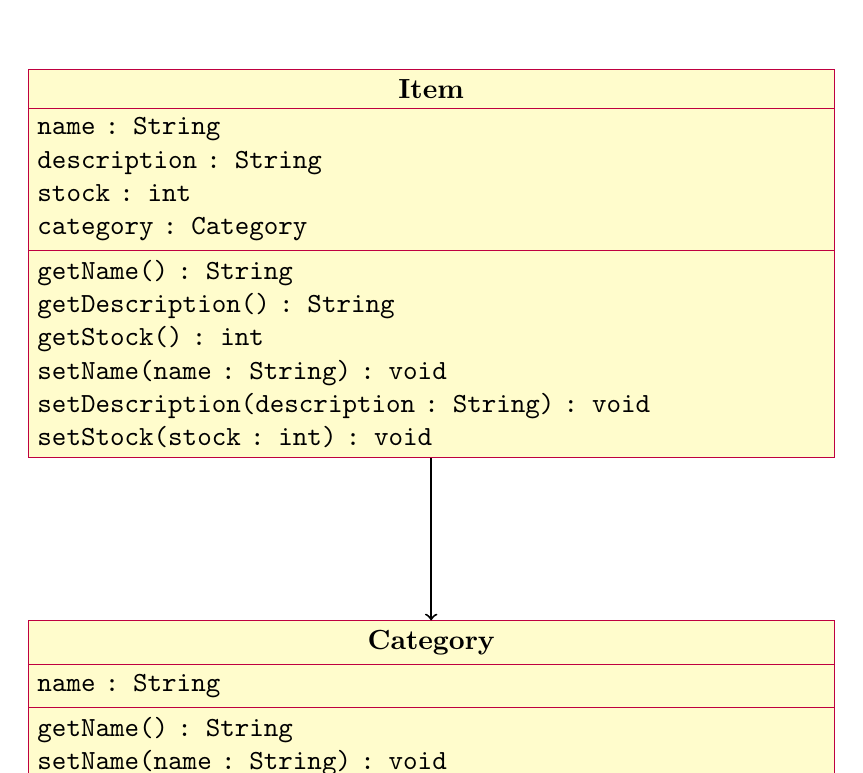
\begin{tikzpicture}
            \begin{class}[text width=10cm]{Item}{0,0}
                \attribute{\texttt{name : String}}
                \attribute{\texttt{description : String}}
                \attribute{\texttt{stock : int}}
                \attribute{\texttt{category : Category}}
                \operation{\texttt{getName() : String}}
                \operation{\texttt{getDescription() : String}}
                \operation{\texttt{getStock() : int}}
                \operation{\texttt{setName(name : String) : void}}
                \operation{\texttt{setDescription(description : String) : void}}
                \operation{\texttt{setStock(stock : int) : void}}
            \end{class}

            \begin{class}[text width=10cm]{Category}{0,-7}
                \attribute{\texttt{name : String}}
                \operation{\texttt{getName() : String}}
                \operation{\texttt{setName(name : String) : void}}
            \end{class}

            \draw [connector] (Item) -- (Category);
        \end{tikzpicture}
    }
\end{itemize}

\end{document}

